%%----------------------------------------------------------------------------
%% Presentatie HoGent Bedrijf en Organisatie
%%----------------------------------------------------------------------------
%% Auteur: Bert Van Vreckem [bert.vanvreckem@hogent.be]

\documentclass{beamer}

%==============================================================================
% Aanloop
%==============================================================================

%---------- Packages ----------------------------------------------------------
\usepackage{etex}
\usepackage{graphicx,multicol}
\usepackage{comment,enumerate,hyperref}
\usepackage{amsmath,amsfonts,amssymb}
\usepackage{tikz}
\usepackage[dutch]{babel}
\usepackage[utf8]{inputenc}
\usepackage{multirow}
\usepackage{eurosym}
\usepackage{listings}
\usepackage[T1]{fontenc}
\usepackage{lmodern}
\usepackage{textcomp}
\usepackage{framed}
\usepackage{wrapfig}
\usepackage{pgf-pie}
\usepackage{pgfplots}
\usepackage{booktabs}
\usepackage{pgfplotstable}
\usepackage{changepage}

%---------- Configuratie ------------------------------------------------------

\usetikzlibrary{arrows,shapes,backgrounds,positioning,shadows}
\usetikzlibrary{pgfplots.statistics}


\lstset{ %
  language=R,                     % the language of the code
  float=H,
  basicstyle=\tiny,       % the size of the fonts that are used for the code
  numbers=left,                   % where to put the line-numbers
  numberstyle=\tiny\color{HoGentGrey},  % the style that is used for the line-numbers
  stepnumber=1,                   % the step between two line-numbers. If it's 1, each line
  % will be numbered																
  numbersep=5pt,                  % how far the line-numbers are from the code
  backgroundcolor=\color{white},  % choose the background color. You must add \usepackage{color}
  showspaces=false,               % show spaces adding particular underscores
  showstringspaces=false,         % underline spaces within strings
  showtabs=false,                 % show tabs within strings adding particular underscores
  frame=single,                   % adds a frame around the code
  rulecolor=\color{black},        % if not set, the frame-color may be changed on line-breaks within not-black text (e.g. commens (green here))
  tabsize=2,                      % sets default tabsize to 2 spaces
  captionpos=b,                   % sets the caption-position to bottom
  breaklines=true,                % sets automatic line breaking
  breakatwhitespace=false,        % sets if automatic breaks should only happen at whitespace
  title=\lstname,                 % show the filename of files included with \lstinputlisting;
  % also try caption instead of title
  keywordstyle=\color{HoGentBlue}, % keyword style
  commentstyle=\color{HoGentGrey}, % comment style
  stringstyle=\color{HoGentRed},  % string literal style
  escapeinside={\%*}{*)},         % if you want to add a comment within your code
  morekeywords={*,...}            % if you want to add more keywords to the set
} 

\usetheme{hogent}
\setbeameroption{show notes}

%---------- Commando-definities -----------------------------------------------

\newcommand{\tabitem}{~~\llap{\textbullet}~~}
\renewcommand{\arraystretch}{1.2}

%---------- Info over de presentatie ------------------------------------------

\title[Intro]{Research techniques\\3. Sampling}
\author{Anita Bernard, Jens Buysse, Bert {Van Vreckem}}
\date{AY 2016-2017}

%==============================================================================
% Inhoud presentatie
%==============================================================================

\begin{document}

%---------- Front matter ------------------------------------------------------

% Dia met het HoGent logo
\HoGentLogo

% Titeldia met faculteitslogo
\titleframe

%---------- Inhoud ------------------------------------------------------------

\begin{frame}
  \frametitle{What's on the menu today?}

  \tableofcontents
\end{frame}

\section{Sampling}
\sectionframelogo{USA Today has come out with a new survey. Apparently, three out of every four people make up 75\% of the population\\

  --David Letterman
}

\begin{frame}
  \frametitle{Sample and population}
  Remember our superheroes
  \begin{tikzpicture}[xscale=4,yscale=2]
    \draw (0,2) -- (0,0);
    \foreach \num/\label in {0/0, 0.2/20, .4/40, .6/60, .8/80, 1/100, 1.2/120, 1.4/140, 1.6/160, 1.8/180, 2/200}{%
      \draw (0, \num) -- (2.5, \num);
      \draw[shift={(0, \num)}] (1pt,0pt) -- (-1pt,0pt) node[left] {\scriptsize \label};
    }

    \node[anchor=north] (hero1) at (0.3,1.5)
    {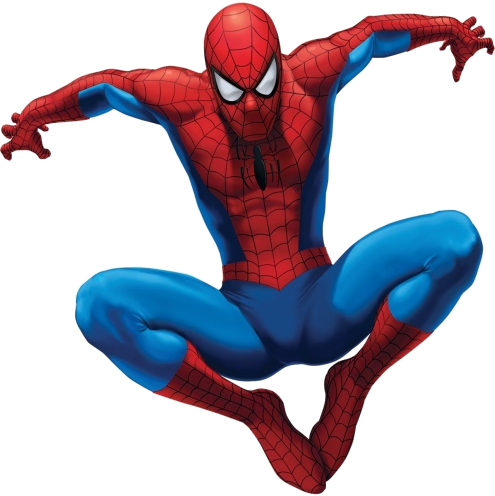
\includegraphics[height=2.9cm]{img/les2-hero-1}};
    \node[anchor=north] (hero2) at (0.8,2.05)
    {
\includegraphics[height=4cm]{img/les2-hero-2}};
    \node[anchor=north] (hero3) at (1.3,1.575)
    {
\includegraphics[height=3.1cm]{img/les2-hero-3}};
    \node[anchor=north] (hero4) at (1.8,2.1)
    {
\includegraphics[height=4.1cm]{img/les2-hero-4}};
    \node[anchor=north] (hero5) at (2.3,1.95)
    {
\includegraphics[height=3.8cm]{img/les2-hero-5}};

    \node (size1) at (0.3, 1.5) {\scriptsize 141 cm};
    \node (size2) at (0.8, 2.1) {\scriptsize 198 cm};
    \node (size3) at (1.3, 1.51) {\scriptsize 143 cm};
    \node (size4) at (1.8, 2.15) {\scriptsize 201 cm};
    \node (size5) at (2.3, 1.95) {\scriptsize 184 cm};
  \end{tikzpicture}
\end{frame}

\begin{frame}
  \frametitle{Sample and population}

  \begin{figure}
    \centering
    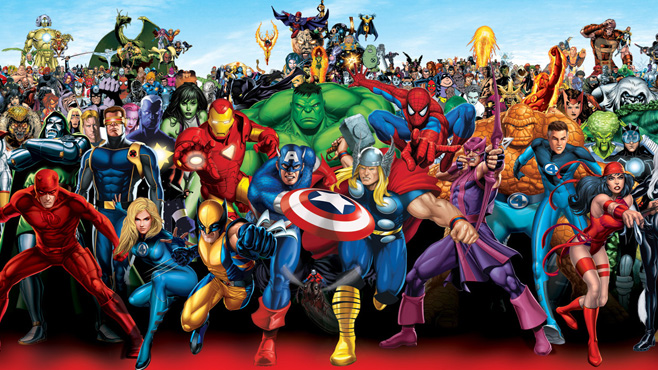
\includegraphics[width=1.00\textwidth]{img/les5-heroes.jpg}
    \label{fig:les5-heroes}
  \end{figure}

\end{frame}

\begin{frame}
  \frametitle{Sample and population}
  \brightbox{ The set of all objects that are being researched is called the \textcolor{HoGentAccent6}{population}.}

  \brightbox{ A subset from the population that is being researched more closely is called a \textcolor{HoGentAccent6}{sample}.}

  \begin{center}
    \begin{tikzpicture}
      \fill[HoGentAccent4] (2,2) ellipse (4cm and 2 cm) ;
      \fill[HoGentAccent2] (2,2) ellipse (2cm and 1cm) ;
      \node[draw=none,minimum size=1cm,inner sep=0pt] at (3,0.5) {population};
      \node[draw=none,minimum size=1cm,inner sep=0pt] at (3,2) {sample};
    \end{tikzpicture}
  \end{center}
\end{frame}

\begin{frame}
  \frametitle{Sampling methods}
  \begin{center}
    \begin{tikzpicture}[
        auto, thick, ->, >=stealth', shorten >=1pt, node distance=2cm,
        fase/.style={ shape=rectangle, fill=HoGentFBO, text=white, draw}
      ]

    \node[fase] (1) { Definition of the population};
    \node[fase] (2) [below of=1] { Specifying a sampling frame };
    \node[fase] (3) [below of=2] { Time/budget considerations };

    \draw (1) -- (2);
    \draw (2) -- (3);
    \end{tikzpicture}
  \end{center}

\end{frame}

\begin{frame}
  \frametitle{Sampling methods}

  \begin{description}
    \item[Random sample] each element from the population has an equal probability of being selected into the sample (probability sampling)
    \item[Non-probability sampling] the sample is selected according to some other methodology that is usually more convenient
  \end{description}

  \begin{center}
    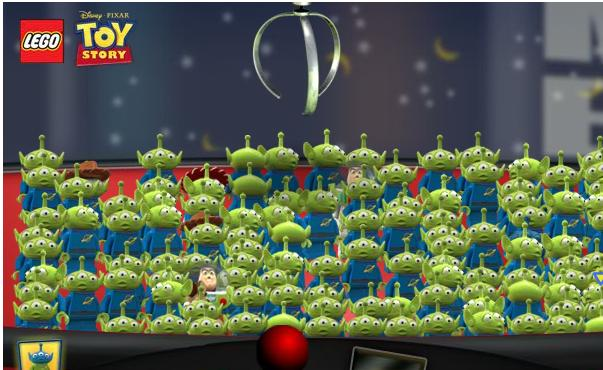
\includegraphics[width=.5\textwidth]{img/les4-aselect}
  \end{center}
\end{frame}

\begin{frame}
  \frametitle{Stratified samples}

  \begin{center}
    \begin{tabular}{l|cccc|c}
      & \multicolumn{4}{c|}{\textbf{Age}} & \\
      Gender & $\le 18$ & $]18,25]$ & $]25, 40]$ & $> 40$ & Total\\
      \hline
      Female & 500 & 1500 & 1000 & 250 & 3250 \\
      Male   & 400 & 1200 & 800 & 160 & 2560\\
      \hline
      Total  & 900 & 2700 & 1800 & 410 & 5810
    \end{tabular}

    \vspace{1cm}

    \pause
    \begin{tabular}{l|cccc|c}
      & \multicolumn{4}{c|}{\textbf{Age}} & \\
      Gender & $\le 18$ & $]18,25]$ & $]25, 40]$ & $> 40$ & Total\\
      \hline
      Female & 50 & 150 & 100 & 25 & 325 \\
      Male   & 40 & 120 & 80 & 16 & 256\\
      \hline
      Total & 90 & 270 & 180 & 41 & 581
    \end{tabular}

  \end{center}
\end{frame}

\begin{frame}
  \frametitle{Sample errors}

  \begin{itemize}
    \item<+-> Random sampling errors
      \begin{itemize}
        \item Random variations in the sampling due to random selection
      \end{itemize}
    \item<+-> Selection bias
      \begin{itemize}
        \item e.g.~online survey will not reach people without internet access
      \end{itemize}
    \item<+-> Random non-sampling errors
      \begin{itemize}
        \item E.g.~respondent checked the wrong answer by mistake
      \end{itemize}
    \item<+-> Systematic non-sampling errors
      \begin{itemize}
        \item E.g.~respondents that have positive affinity with the subject are more likely to participate.
      \end{itemize}
  \end{itemize}
\end{frame}

\begin{frame}
  \frametitle{Variance and standard deviation of a sample}

  \begin{center}
    Adapted formula:

    \begin{equation*}
    s^2 = \frac{1}{\alert{n-1}} \sum_{i=1}^{n} (\overline{x} - x_i)^2
    \end{equation*}

    It is possible to prove mathematically why this is better, but we will study this empirically.

    \vfill

    Java applet: \url{http://www.uvm.edu/~dhowell/SeeingStatisticsApplets/N-1.html}
    \vfill
    R-script: \href{https://github.com/HoGentTIN/research-techniques-course/blob/master/syllabus/data/sample-variance.R}{syllabus/data/sample-variance.R}
  \end{center}
\end{frame}

\section{Probability distribution of a sample}

\begin{frame}
  \frametitle{Recap from probability theory}

  \begin{itemize}
    \item Sample space
    \item Outcome
    \item Event
    \item Probability space
  \end{itemize}

  \vfill

  \hfill 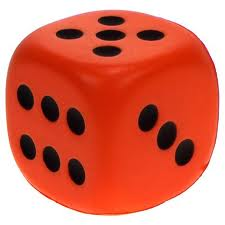
\includegraphics[width=.2\textwidth]{img/les04-dobbelsteen}
\end{frame}

\begin{frame}
  \frametitle{Probability distribution for a single die}

  What is the probability to throw a specific number with a single die?

  \begin{center}
    \begin{tabular}{|c|c|c|c|c|c|}
      \hline
      1&2&3&4&5&6\\
      \hline
      \onslide<2->{$\frac{1}{6}}$ &\onslide<2->{$\frac{1}{6}}$ &\onslide<2->{$\frac{1}{6}}$ &\onslide<2->{$\frac{1}{6}}$ &\onslide<2->{$\frac{1}{6}}$ &     \onslide<2->{$\frac{1}{6}}$ \\
      \hline

    \end{tabular}
  \end{center}

  \onslide<2->{%
  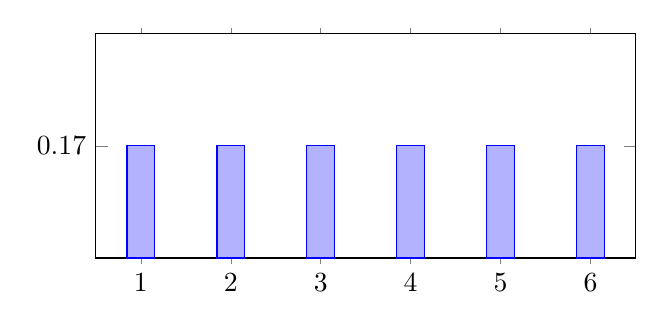
\begin{tikzpicture}
    \begin{axis}[ybar,ytick=data, anchor=north, yscale=.5]
      \addplot
      coordinates {
        (1, 1/6)
        (2, 1/6)
        (3, 1/6)
        (4, 1/6)
        (5, 1/6)
        (6, 1/6)};
    \end{axis}
  \end{tikzpicture}}
\end{frame}

\begin{frame}
  \frametitle{Probability distribution for two dice}

  \begin{center}
    \begin{tabular}{|c|c|c|c|c|c|c|c|c|c|c|c|}
      \hline
      2&3&4&5&6&7&8&9&10&11&12\\
      \hline
      \onslide<2->{$\frac{1}{36}}$ &\onslide<2->{$\frac{2}{36}}$ &\onslide<2->{$\frac{3}{36}}$ &\onslide<2->{$\frac{4}{36}}$ &\onslide<2->{$\frac{5}{36}}$ & \onslide<2->{$\frac{6}{36}}$ & \onslide<2->{$\frac{5}{36}}$ &\onslide<2->{$\frac{4}{36}}$ & \onslide<2->{$\frac{3}{36}}$ &\onslide<2->{$\frac{2}{36}}$ &\onslide<2->{$\frac{1}{36}}$ \\
      \hline

    \end{tabular}
  \end{center}

  \onslide<2->{%
  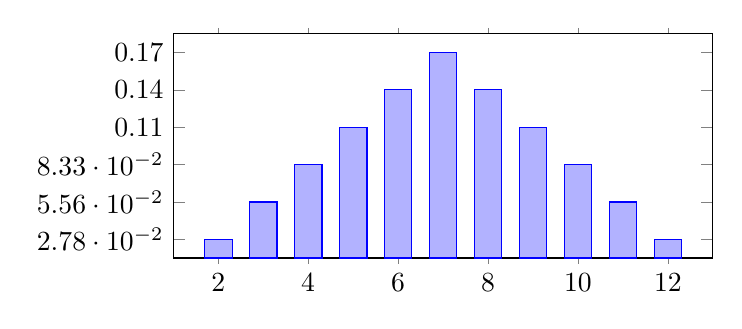
\begin{tikzpicture}
    \begin{axis}[ybar,ytick=data, anchor=north, yscale=.5]
      \addplot
      coordinates {
        (2, 1/36)
        (3, 2/36)
        (4, 3/36)
        (5, 4/36)
        (6, 5/36)
        (7, 6/36)
        (8, 5/36)
        (9, 4/36)
        (10, 3/36)
        (11, 2/36)
        (12, 1/36)
      };

    \end{axis}
  \end{tikzpicture}}

\end{frame}

  \pgfmathdeclarefunction{gauss}{2}{%
    \pgfmathparse{1/(#2*sqrt(2*pi))*exp(-((x-#1)^2)/(2*#2^2))}%
  }

\begin{frame}
  \frametitle{Continuous probability distribution}

  The probability distribution of Superman's reaction time:

  \vspace{1cm}

  \begin{tikzpicture}
\begin{axis}[
  domain=0:10, samples=100,
  axis lines*=left, xlabel=$x$, ylabel=$y$,
  every axis y label/.style={at=(current axis.above origin),anchor=south},
  every axis x label/.style={at=(current axis.right of origin),anchor=west},
  height=5cm, width=12cm,
  xtick={5,3.5,6.5}, ytick=\empty,
  enlargelimits=false, clip=false, axis on top,
  grid = major
  ]
  \addplot [fill=cyan!20, draw=none, domain=0:9] {gauss(5,1.5)} \closedcycle;
  \draw [yshift=-0.6cm, latex-latex](axis cs:3.5,0) -- node [fill=white] {$\sigma$} (axis cs:6.5,0);
  \end{axis}
  \end{tikzpicture}
  \hfill
\includegraphics[width=1.5cm]{img/les2-hero-3}
\end{frame}

\begin{frame}
  \frametitle{Standard normal distribution}

  % Source: http://johncanning.net/wp/?p=1202
  \begin{center}
    \begin{tikzpicture}
      \begin{axis}[
          no markers, domain=0:10, samples=100,
          axis lines*=left,height=6cm, width=10cm,
          xtick={-3, -2, -1, 0, 1, 2, 3}, ytick=\empty,
          enlargelimits=false, clip=false, axis on top,
          grid = major
        ]
        \addplot [smooth,fill=cyan!20, draw=none, domain=-3:3] {gauss(0,1)} \closedcycle;
        \addplot [smooth,fill=orange!20, draw=none, domain=-3:-2] {gauss(0,1)} \closedcycle;
        \addplot [smooth,fill=orange!20, draw=none, domain=2:3] {gauss(0,1)} \closedcycle;
        \addplot [smooth,fill=blue!20, draw=none, domain=-2:-1] {gauss(0,1)} \closedcycle;
        \addplot [smooth,fill=blue!20, draw=none, domain=1:2] {gauss(0,1)} \closedcycle;
        \addplot[<->] coordinates {(-1,0.4) (1,0.4)};
        \addplot[<->] coordinates {(-2,0.3) (2,0.3)};
        \addplot[<->] coordinates {(-3,0.2) (3,0.2)};
        \node[coordinate, pin={68.2\%}] at (axis cs: 0, 0.35){};
        \node[coordinate, pin={95\%}] at (axis cs: 0, 0.25){};
        \node[coordinate, pin={99.7\%}] at (axis cs: 0, 0.15){};
        \node[coordinate, pin={34.1\%}] at (axis cs: -0.5, 0){};
        \node[coordinate, pin={34.1\%}] at (axis cs: 0.5, 0){};
        \node[coordinate, pin={13.6\%}] at (axis cs: 1.5, 0){};
        \node[coordinate, pin={13.6\%}] at (axis cs: -1.5, 0){};
        \node[coordinate, pin={2.1\%}] at (axis cs: 2.5, 0){};
        \node[coordinate, pin={2.1\%}] at (axis cs: -2.5, 0){};
      \end{axis}
    \end{tikzpicture}
  \end{center}
\end{frame}

\begin{frame}
  \frametitle{What is the probability that\dots}

  Superman's reaction speed is longer than 6.5 milliseconds?

  \vspace{2cm}

  \begin{itemize}
    \item $z$-table with left tail probabilities, e.g.~\url{http://sixsigmastudyguide.com/wp-content/uploads/2014/04/z-table.jpg}
    \item Rule of symmetry
    \item 100\% probability rule
  \end{itemize}
\end{frame}

\begin{frame}[fragile]
  \frametitle{Most important R functions}
  
  A normal distribution with mean \texttt{m} and standard deviation \texttt{s}:
  \vfill
  \centering
  \begin{tabular}{ll}
  	\textbf{Function}     & \textbf{Return value}                       \\ \hline
  	\verb|pnorm(x, m, s)| & Left tail probability, $P(X<\mathtt{x})$         \\
  	\verb|dnorm(x, m, s)| & Height of the Gauss curve at \texttt{x} \\
  	\verb|qnorm(p, m, s)| & Under what limit will \texttt{p}\% of the   \\
  	                      & observations be situated?                        \\
  	\verb|rnorm(n, m, s)| & Generate \texttt{n} normally distributed randon numbers
  \end{tabular}
  \vfill
  Default value for \texttt{m} is 1, for \texttt{s} is 0 (standard normal distribution)
\end{frame}

\begin{frame}
  \frametitle{Application}

  What is the probability that Superman's reaction time is

  \begin{enumerate}
    \item Less than 4 ms?
    \item More than 7 ms?
    \item Less than 3 ms?
    \item Between 2 and 6.5 ms?
    \item Under what time limit is 80\% of his reaction times?
  \end{enumerate}
\end{frame}

\begin{frame}
  \frametitle{Question 3: $P(X<3)$}

  \begin{tikzpicture}
  \begin{axis}[no markers,domain=-4:4,axis lines*=left,yscale=.7,enlargelimits=false,clip=false]
    \addplot[very thick,smooth,draw=HoGentFBO]{gauss(0, 1)};
    \addplot[smooth,fill=black!20, draw=black, domain=-4:-4/3] {gauss(0,1)} \closedcycle;

    \node at (axis cs: -1.33, -.05) {\small -1.33};
  \end{axis}
  \end{tikzpicture}
\end{frame}

\begin{frame}
  \frametitle{Question 4: $P(2<X<6,5)$}

  \begin{tikzpicture}
  \begin{axis}[no markers,domain=-4:4,axis lines*=left,yscale=.7,enlargelimits=false,clip=false]
    \addplot[very thick,smooth,draw=HoGentFBO]{gauss(0, 1)};
    \addplot[smooth,fill=black!20, draw=black, domain=-2:1] {gauss(0,1)} \closedcycle;

    \node at (axis cs: 1, -.05) {\small 1};
  \end{axis}
  \end{tikzpicture}
\end{frame}

\begin{frame}
  \frametitle{Question 5}

  For what value of $x$ is $P(X<x) = 80\%$?

  \vfill

  \begin{tikzpicture}
  \begin{axis}[no markers,domain=-4:4,axis lines*=left,yscale=.7,enlargelimits=false,clip=false]
    \addplot[very thick,smooth,draw=HoGentFBO]{gauss(0, 1)};
    \addplot[smooth,fill=black!20, draw=black, domain=-4:.84] {gauss(0,1)} \closedcycle;

    \node at (axis cs: .84, -.05) {\small .84};
  \end{axis}
  \end{tikzpicture}
\end{frame}

\section{The central limit theorem}
\sectionframelogo{}


\begin{frame}
  \frametitle{The central limit theorem}

  \brightbox{If the sample size is sufficiently large, then the probability distribution of the arithmetic mean will be approximately normally distributed, regardless of the underlying distribution.}

  \vfill

  \begin{columns}[c]
    \column{.33\textwidth}
    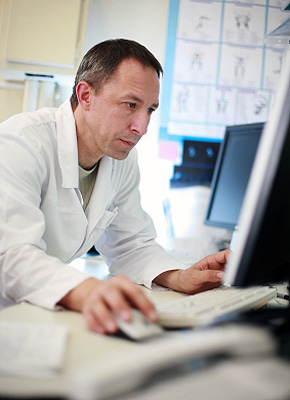
\includegraphics[width=2cm]{img/les4-centrlimiet}
    \column{.33\textwidth}
    \begin{itemize}
      \item 1 test
      \item 25 tests
      \item 100 tests
    \end{itemize}
    \column{.33\textwidth}
    
\includegraphics[width=2cm]{img/les2-hero-3}
  \end{columns}

\end{frame}

\begin{frame}
  \frametitle{The central limit theorem}

  Consider a random sample of $n$ observations from a population with expected value $\mu$ and standard deviation $\sigma$. If $n$ is sufficiently large, the probability of $\overline{x}$ will approximate a normal distribution with mean $\mu_{\overline{x}} = \mu$ and standard deviation $\sigma_{\overline{x}} = \frac{\sigma}{\sqrt{n}}$. The larger the sample, the better the approximation of $\overline{x}$ will be.
\end{frame}

\section{From sample to population}
\sectionframelogo{}

\begin{frame}
  \frametitle{Point estimate}
  \brightbox{A \textcolor{HoGentYellow}{point estimate} for a population parameter is a formula for estimating that parameter from the sample.}

\end{frame}

\subsection{Confidence intervals}

\begin{frame}
  \frametitle{Confidence interval}

  \brightbox{A \textcolor{HoGentYellow}{confidence interval} for a population parameter is a formula for estimating an interval that will contain the value of that parameter with a specific \textcolor{HoGentYellow}{confidence level}. }

\end{frame}

\subsection{Confidence interval for large samples}

\begin{frame}
  \frametitle{Confidence interval for large samples}
  \begin{figure}[t]
\centering
\begin{tikzpicture}
\begin{axis}[
  domain=-3:3, samples=100,
  axis lines*=left, xlabel=$z$,
  every axis y label/.style={at=(current axis.above origin),anchor=south},
  every axis x label/.style={at=(current axis.right of origin),anchor=west},
  height=5cm, width=12cm,
  xtick={-1.96,0,1.96}, ytick=\empty,
  enlargelimits=false, clip=false, axis on top,
  grid = major
  ]
  \addplot [fill=cyan!20, draw=none, domain=-3:3] {gauss(0,1)} \closedcycle;
  \draw [yshift=-0.6cm, latex-latex](axis cs:-1.96,0) -- node [fill=white] {$\sigma$} (axis cs:1.96,0);
\end{axis}
\end{tikzpicture}
\caption{Standard normal distribution with a confidence interval for a confidence level of 95\%.}
\label{fig:verdelingStandaardnormaal}
\end{figure}
\end{frame}

\subsection{Confidence interval for small samples}
\begin{frame}
  \frametitle{Confidence interval for small samples}
  Instead of

\[ z = \frac{\overline{x} - \mu}{\frac{\sigma}{\sqrt{n}}} \]

we use

\[ t = \frac{\overline{x} - \mu}{\frac{s}{\sqrt{n}}} \]

  with $t$ the $t$-score from Student's $t$-distribution.
\end{frame}

\begin{frame}
  \frametitle{Confidence interval for small samples}

  To determine the confidence interval for the mean based on a small sample, we calculate:

  \[ \overline{x} \pm t_{\frac{\alpha}{2}}(\frac{s}{\sqrt{n}}) \]

  with $t_{\frac{\alpha}{2}}$ is based on $(n-1)$ degrees of freedom. We assume that the sample is random and the population is approximately randomly distributed.
\end{frame}


\begin{frame}[fragile]
\frametitle{Student's $t$-distribution in R}

For a $t$-distribution with \texttt{df} degrees of freedom:
\vfill
\centering
\begin{tabular}{ll}
	\textbf{Function} & \textbf{Return value}                                    \\ \hline
	\verb|pt(x, df)| & Left tail probability, $P(X<\mathtt{x})$                  \\
	\verb|dt(x, df)| & Height of the curve at \texttt{x}                     \\
	\verb|qt(p, df)| & Under what limit will \texttt{p}\% of the     \\
	                 & obsevations be situated?                             \\
	\verb|rt(n, df)| & Generate \texttt{n} random numbers with this distribution
\end{tabular}

\end{frame}

\subsection{Confidence interval for a fraction}
\begin{frame}
  \frametitle{Confidence interval for a fraction}
  \[ \overline{p} = \frac{\textnormal{number of successes}}{n} \]
  \begin{itemize}
  \item The expected value of the probability distribution of $\overline{p}$ is $p$.
  \item The stdev of the probability distribution of  $\overline{p}$ is $\sqrt{\frac{pq}{n}}$
  \item For large samples, $\overline{p}$ is approximately normally distributed
\end{itemize}

Since $\overline{p}$ is a sample mean of the number of successes, this allows us to draw a confidence interval analogous to the previously discussed interval estimate of $\mu$ for large samples.

  \[ \overline{p} \pm z_{\frac{\alpha}{2}} \sqrt{\frac{\overline{p}\overline{q}}{n}} \]
  with $\overline{p} = \frac{x}{n}$ en $\overline{q} = 1- \overline{p}$

\end{frame}

\end{document}
